%%%%%%%%%%%%%%%%%%%%%%%%%%%%%%%%%%%%%%%%%%%%%%%%%%%%%%%%%%%%%%%%%%%%%%
% Overleaf (WriteLaTeX) Example: Molecular Chemistry Presentation
%
% Source: http://www.overleaf.com
%
% In these slides we show how Overleaf can be used with standard 
% chemistry packages to easily create professional presentations.
% 
% Feel free to distribute this example, but please keep the referral
% to overleaf.com
% 
%%%%%%%%%%%%%%%%%%%%%%%%%%%%%%%%%%%%%%%%%%%%%%%%%%%%%%%%%%%%%%%%%%%%%%

\documentclass{beamer}

\mode<presentation>
{
  \usetheme{Madrid}       % or try default, Darmstadt, Warsaw, ...
  \usecolortheme{default} % or try albatross, beaver, crane, ...
  \usefonttheme{default}    % or try default, structurebold, ...
  \setbeamertemplate{navigation symbols}{}
  \setbeamertemplate{caption}[numbered]
} 

\usepackage[english]{babel}
\usepackage[utf8x]{inputenc}
\usepackage{chemfig}
\usepackage[version=3]{mhchem}

\usepackage{hyperref}
  \hypersetup{colorlinks=true}
  \hypersetup{urlcolor=blue}
  \hypersetup{linkcolor = .}
\usepackage{xcolor}
\usepackage{siunitx}
  \sisetup{separate-uncertainty = true}
\usepackage{physics}
\usepackage[font=small,labelfont=bf]{caption}
\usepackage{subcaption}
\usepackage[en-GB]{datetime2}
\usepackage{overpic}
\usepackage{feynmp}
\DeclareGraphicsRule{*}{mps}{*}{}

\usepackage{scalerel}
\newcommand{\mylbrace}[2]{\vspace{#2pt}\hspace{6pt}\scaleleftright[\dimexpr5pt+#1\dimexpr0.06pt]{\lbrace}{\rule[\dimexpr2pt-#1\dimexpr0.5pt]{-4pt}{#1pt}}{.}}
\newcommand{\myrbrace}[2]{\vspace{#2pt}\scaleleftright[\dimexpr5pt+#1\dimexpr0.06pt]{.}{\rule[\dimexpr2pt-#1\dimexpr0.5pt]{-4pt}{#1pt}}{\rbrace}\hspace{6pt}}

% Here's where the presentation starts, with the info for the title slide
\title[BESIII Oxford]{BESIII Oxford Group Meeting}
\author{Martin Tat}
\institute{Oxford LHCb}
\date{30th April 2021}

\titlegraphic{
\includegraphics[width = 5cm, height = 3.8cm]{lhcb.jpg}\hspace{1cm}~%
              
\includegraphics[width = 5cm, height = 3.8cm]{bes3.jpg}}

\begin{document}

\begin{frame}
  \titlepage
\end{frame}

% These three lines create an automatically generated table of contents.
%\begin{frame}{Outline}
%  \tableofcontents
%\end{frame}

\section{Intorduction}
\begin{frame}{Introduction}
  \begin{itemize}
    \setlength\itemsep{2em}
    \item{$D\to K^+K^-\pi^+\pi^-$ analysis}
    \item{Previously:}
    \begin{itemize}
      \item{Obtained ST yield from fit to $m_\text{BC}$}
      \item{$KK\pi\pi$, $KK$, $\pi\pi$}
    \end{itemize}
    \item{Current progress:}
    \begin{itemize}
      \item{Obtained ST yield for $K\pi$, $K\pi\pi^0$, $\pi\pi\pi^0$, $K_S\pi^0$, $K_S\pi^0\pi^0$, $K_S\eta$}
      \item{Obtained DT yield for $KK$, $K_S\pi^0$, $K\pi$ using sideband background subraction}
    \end{itemize}
  \end{itemize}
\end{frame}

\section{Single tag yields}
\begin{frame}{$\pi\pi\pi^0$ and $K_S\pi^0$ ST yield}
  \begin{figure}
    \centering
    \begin{subfigure}{0.5\textwidth}
      \centering
      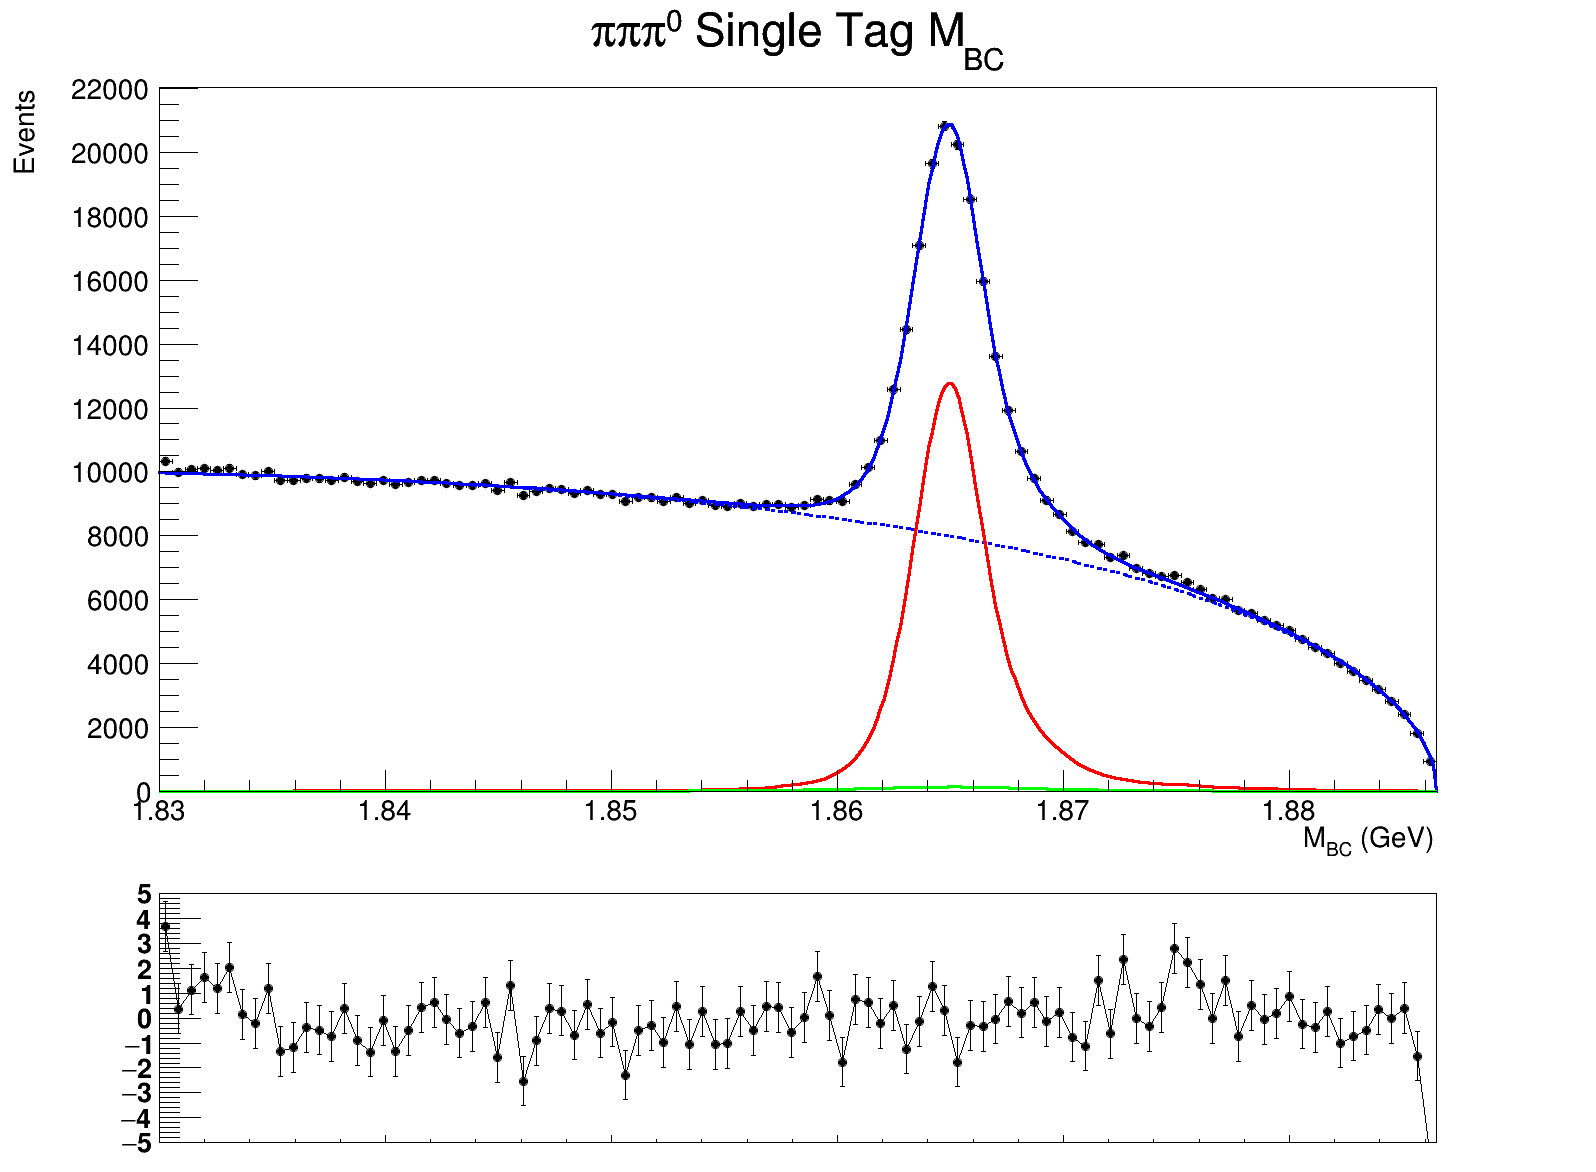
\includegraphics[width=\textwidth]{pipipi0SingleTagMBCPlot.png}
      \caption{$\pi\pi\pi^0$ $m_\text{BC}$ fit}
    \end{subfigure}%
    \begin{subfigure}{0.5\textwidth}
      \centering
      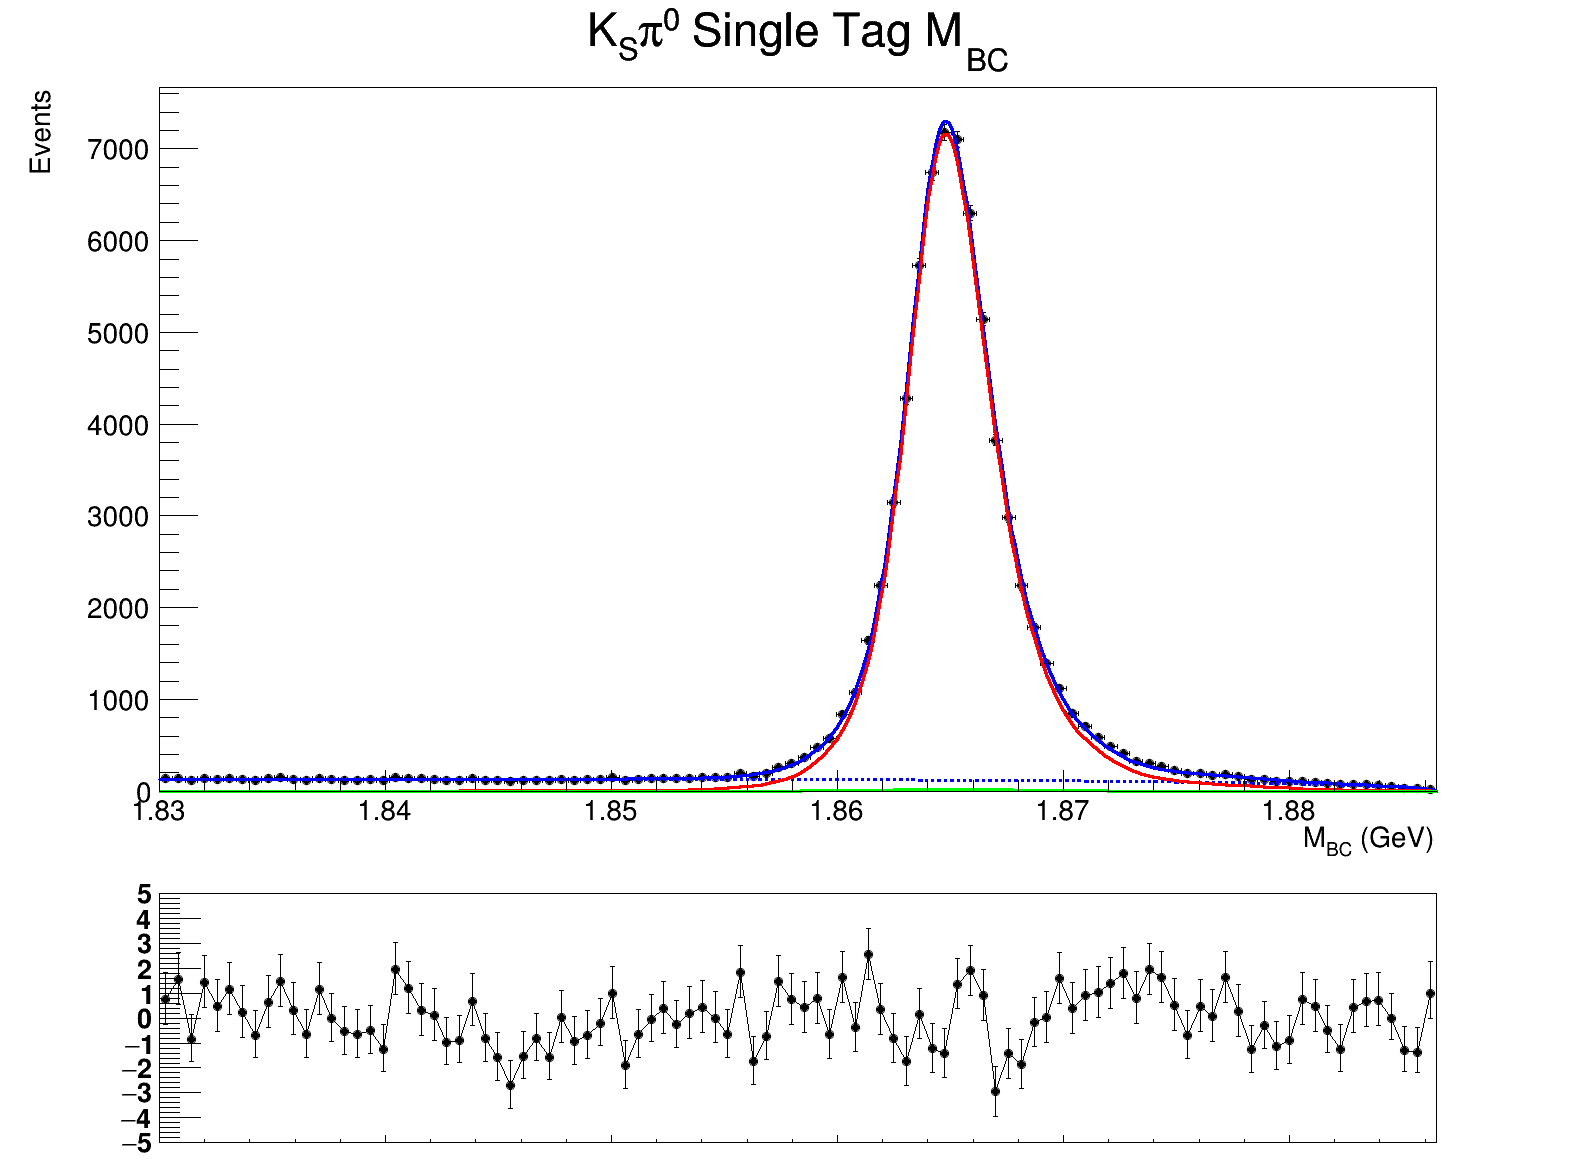
\includegraphics[width=\textwidth]{KSpi0SingleTagMBCPlot.png}
      \caption{$K_S\pi^0$ $m_\text{BC}$ fit}
    \end{subfigure}
  \end{figure}
\end{frame}

\begin{frame}{$K_S\pi^0\pi^0$ and $K_S\eta$ ST yield}
  \begin{figure}
    \centering
    \begin{subfigure}{0.5\textwidth}
      \centering
      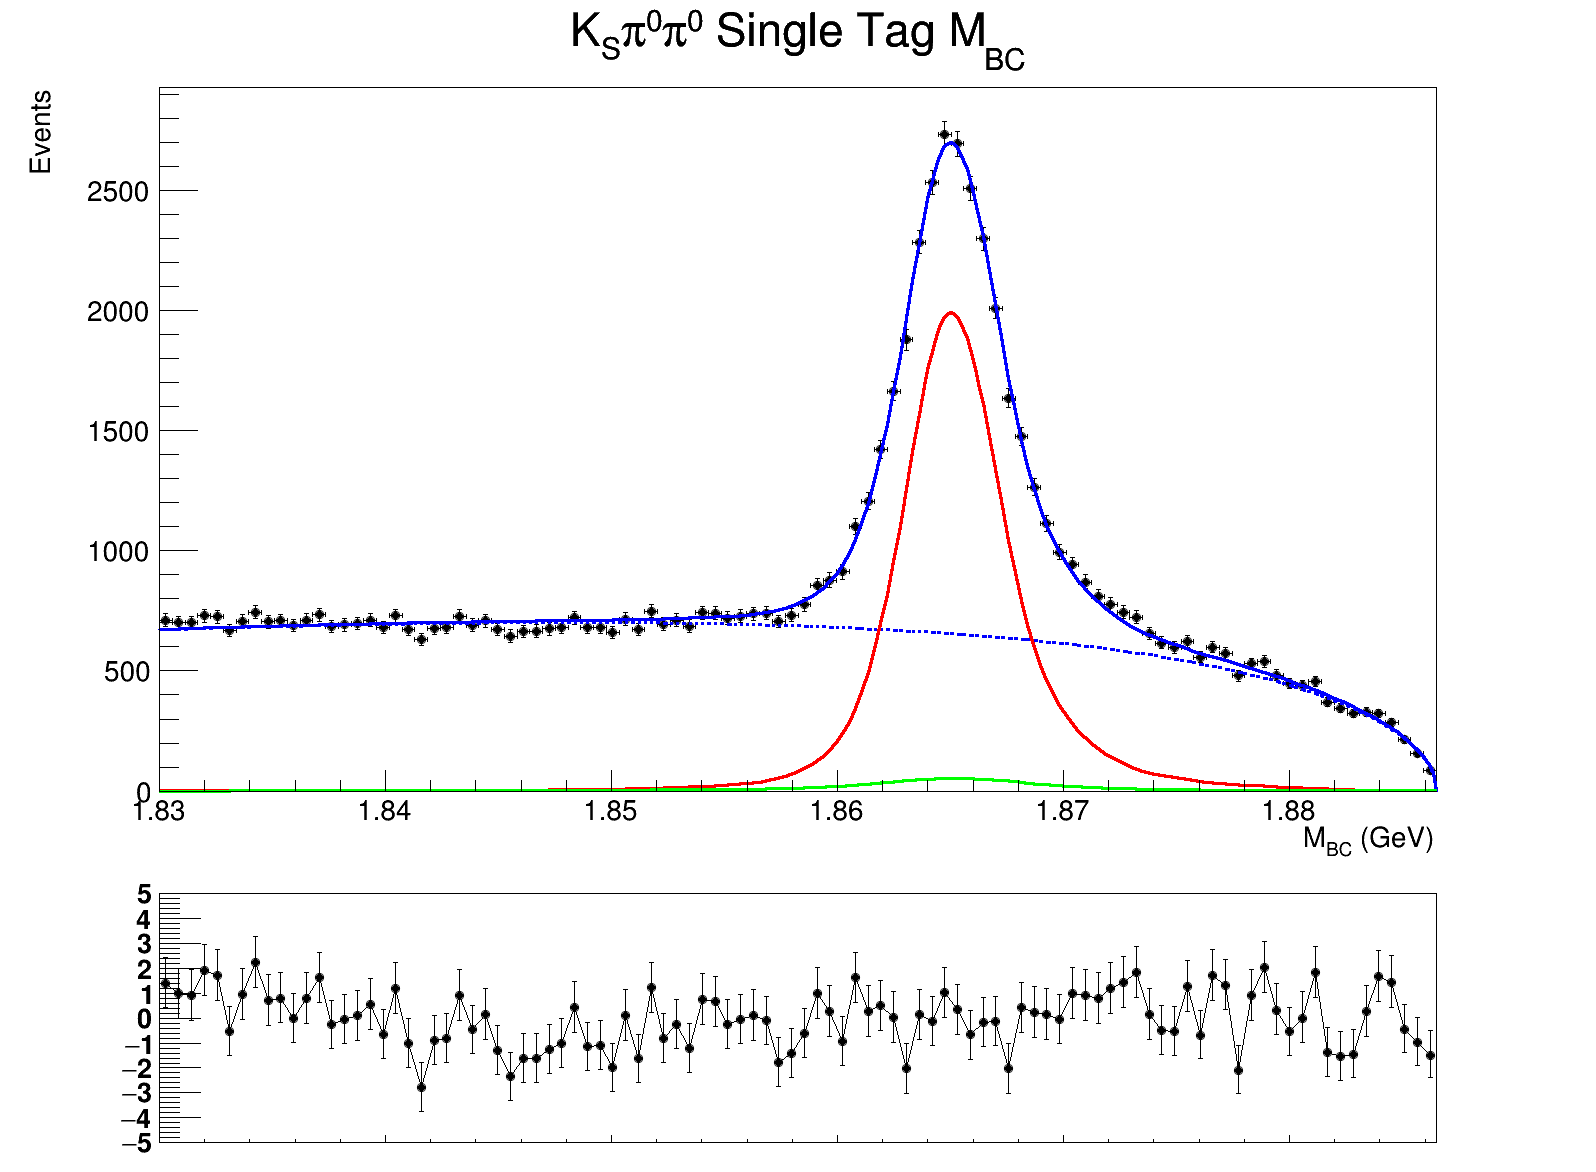
\includegraphics[width=\textwidth]{KSpi0pi0SingleTagMBCPlot.png}
      \caption{$K_S\pi^0\pi^0$ $m_\text{BC}$ fit}
    \end{subfigure}%
    \begin{subfigure}{0.5\textwidth}
      \centering
      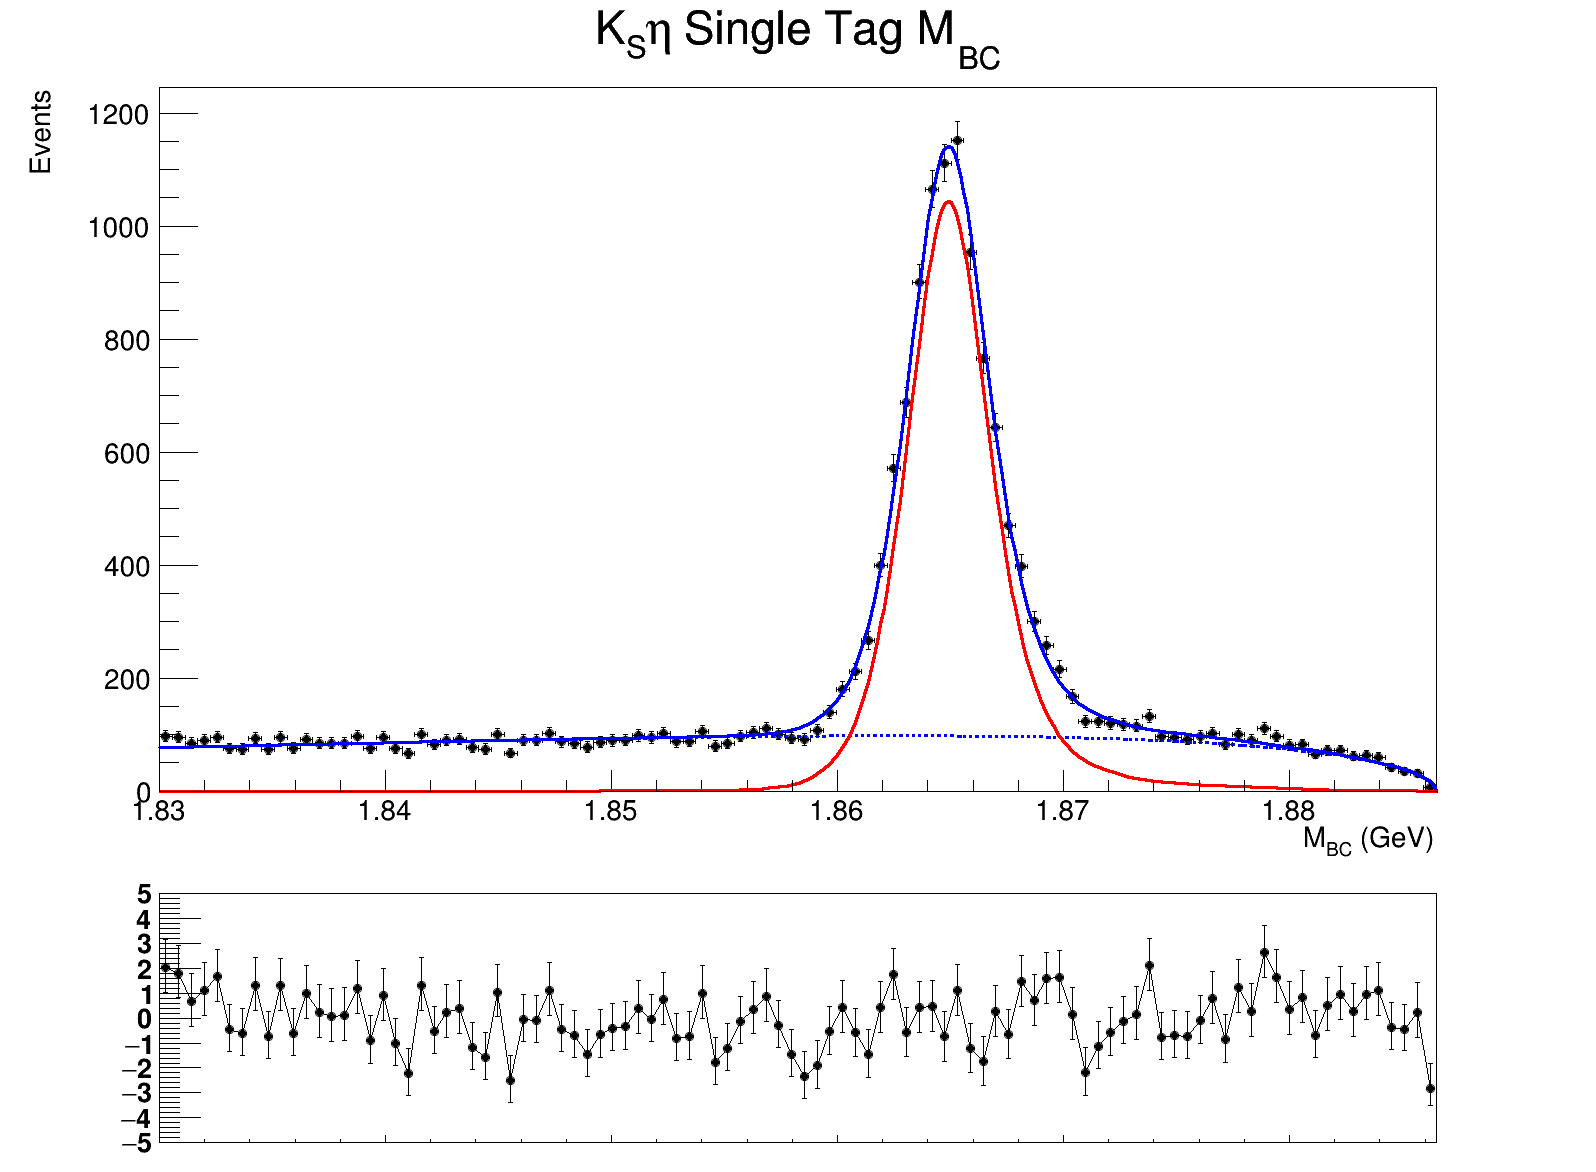
\includegraphics[width=\textwidth]{KSetaSingleTagMBCPlot.png}
      \caption{$K_S\eta$ $m_\text{BC}$ fit}
    \end{subfigure}
  \end{figure}
\end{frame}

\begin{frame}{$K\pi$ and $K\pi\pi^0$ ST yield}
  \begin{figure}
    \centering
    \begin{subfigure}{0.5\textwidth}
      \centering
      \includegraphics[width=\textwidth]{kpiSingleTagMBCPlot.png}
      \caption{$K\pi$ $m_\text{BC}$ fit}
    \end{subfigure}%
    \begin{subfigure}{0.5\textwidth}
      \centering
      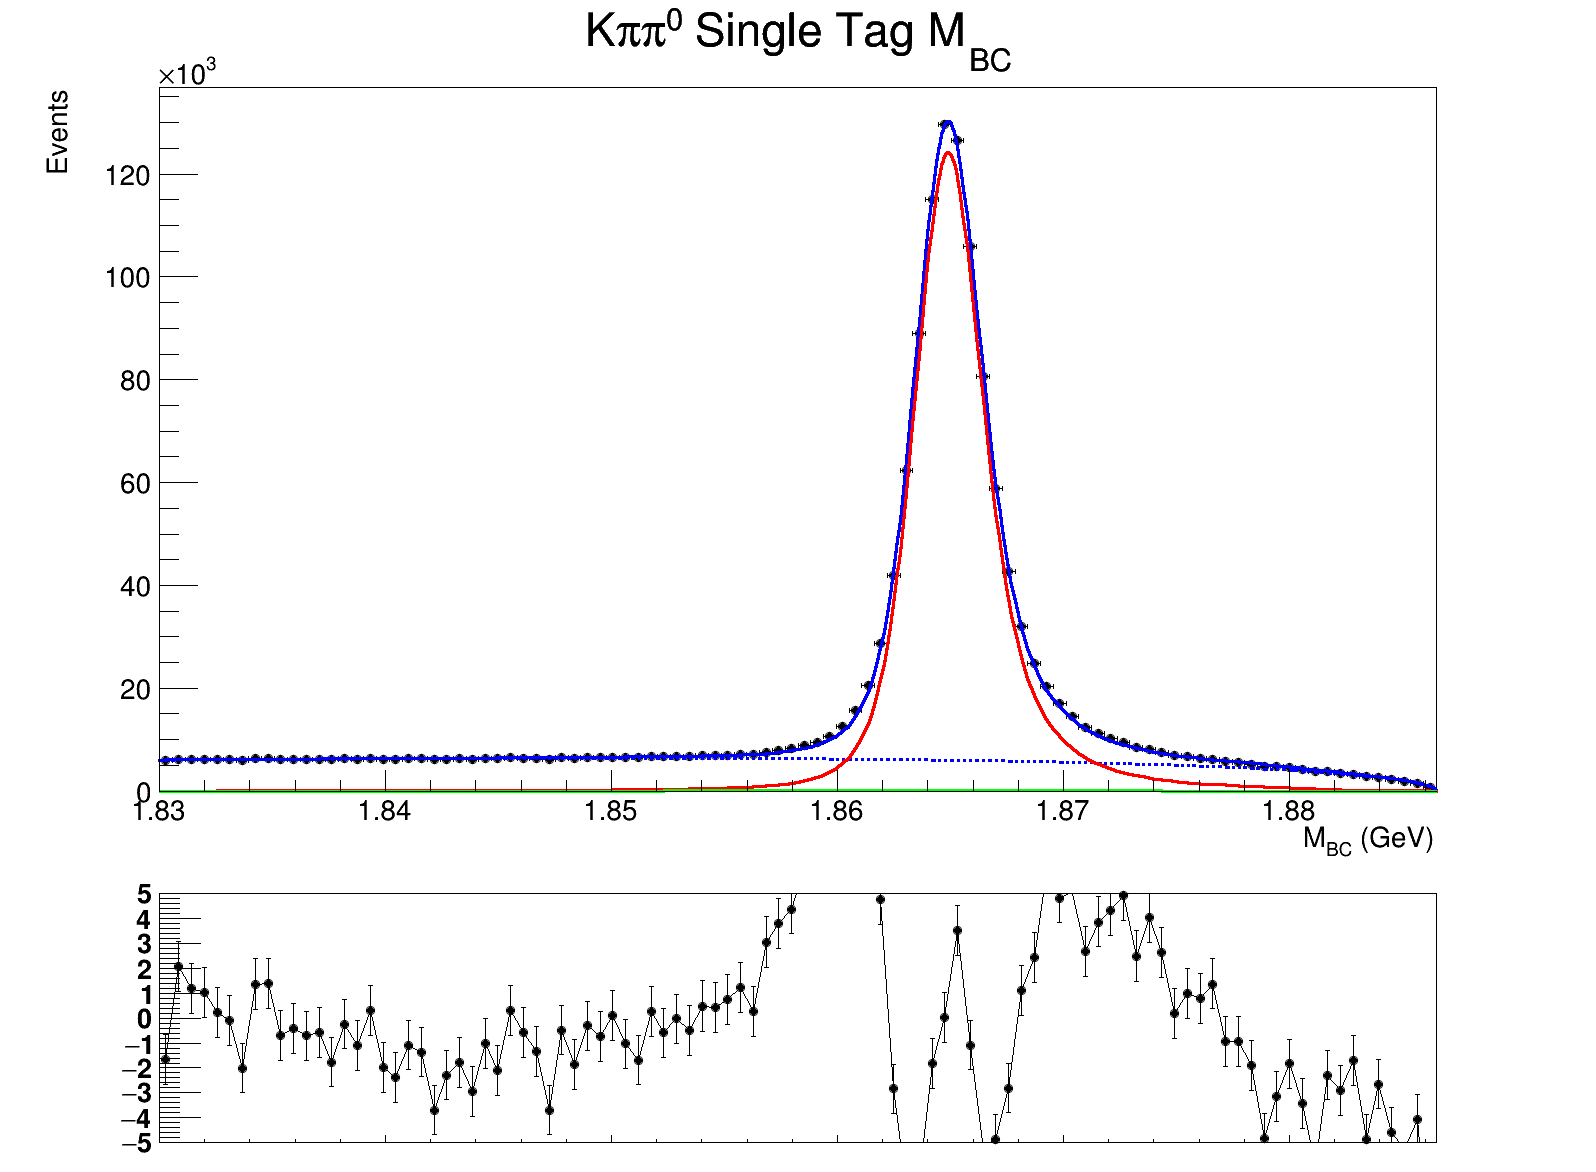
\includegraphics[width=\textwidth]{Kpipi0SingleTagMBCPlot.png}
      \caption{$K\pi\pi^0$ $m_\text{BC}$ fit}
    \end{subfigure}
  \end{figure}
\end{frame}

\begin{frame}{Peaking backgrounds}
  \begin{itemize}
    \item{Shape and yield fixed from inclusive MC}
  \end{itemize}
  \centering
  \def\arraystretch{1.2}%
  \begin{tabular}{ll}
                    & \\
    Tag mode        & Main peaking backgrounds(Yields) \\
    \hline
    $\pi\pi\pi^0$   & $K_S\pi^0$ ($1402$), $K\pi$ ($669$), $K\pi\pi^0$ ($153$) \\
    $K_S\pi^0$      & $\pi\pi\pi^0$ ($227$) \\
    $K_S\pi^0\pi^0$ & $K_SK_S$ ($249$), $K_S\pi^0\gamma$ ($198$), $K_S\eta$ ($244$) \\
                    & $\pi\pi\pi^0\pi^0$ ($149$), $K_S\pi^0$ ($93$), $K_S\pi\pi$ ($57$), $K\pi\pi^0$ ($32$) \\
    $K_S\eta$       & - \\
    $K\pi$          & Other ($95$), $Ke\nu$ ($84$), $K\mu\nu$ ($72$), $\pi\pi\pi^0$ ($62$) \\
    $K\pi\pi^0$     & $\pi\pi\pi^0$ ($807$), $K_S\pi\pi$ ($483$), $K\mu\nu\pi^0$ ($169$) \\
                    & $Ke\nu\pi^0$ ($155$), $K\pi\gamma^\text{FSR}$ ($139$)
    \end{tabular}
\end{frame}

\begin{frame}{Single tag yields}
  \centering
  \def\arraystretch{1.2}%
  \begin{tabular}{ccc}
                    & \\
    Tag mode        & Yield & Result from $K_SKK$ analysis \\
    \hline
    $\pi\pi\pi^0$   & $\SI{97862(530)}{}$ & $\SI{99981(618)}{}$ \\
    $K_S\pi^0$      & $\SI{62357(255)}{}$ & $\SI{65072(281)}{}$ \\
    $K_S\pi^0\pi^0$ & $\SI{19259(195)}{}$ & $\SI{19882(233)}{}$ \\
    $K_S\eta$       & $\SI{8732(106)}{}$ & $\SI{9524(134)}{}$ \\
    $K\pi$          & $\SI{513561(725)}{}$ & $\SI{261221(525)}{}/\SI{266086(525)}{}$ \\
    $K\pi\pi^0$     & $\SI{914620(1044)}{}$ & $\SI{496202(788)}{}/\SI{499481(792)}{}$ \\
    \end{tabular}
\end{frame}

\section{Double tag yields}
\begin{frame}{Double tag yields}
  \begin{itemize}
    \setlength\itemsep{2em}
    \item{$KK\pi\pi$ vs $KK$ (CP even tag)}
    \item{$KK\pi\pi$ vs $K_S\pi^0$ (CP odd tag)}
    \item{$KK\pi\pi$ vs $K\pi$ (flavour tag)}
  \end{itemize}
\end{frame}

\begin{frame}{Sideband background subtraction method}
  \begin{figure}
    \centering
    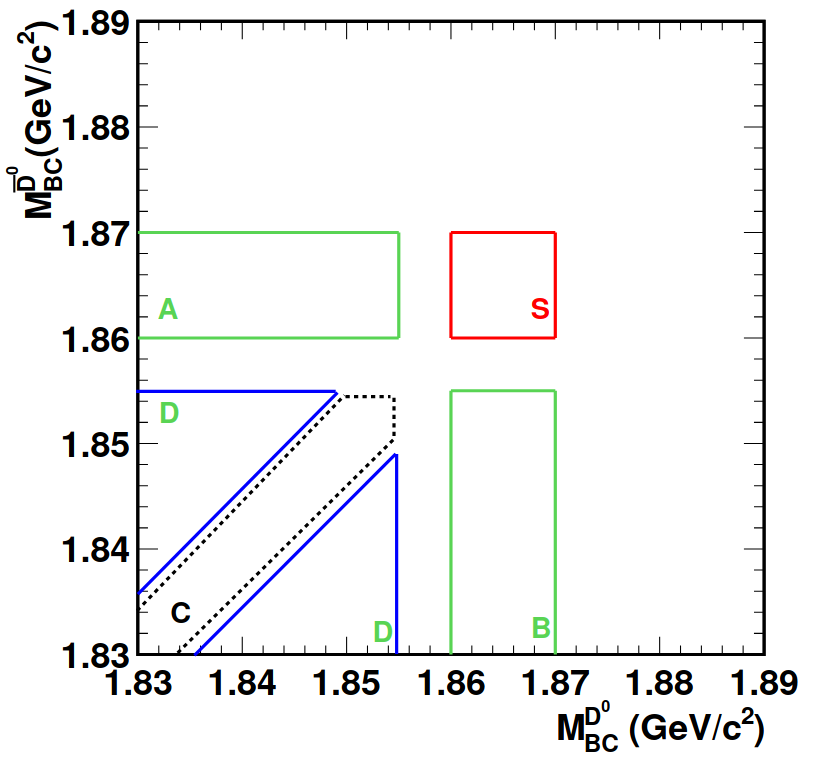
\includegraphics[width=0.5\textwidth]{MBC2D.png}
  \end{figure}
  \begin{equation}
    B = \frac{a_S}{a_D}Y_D + \sum_{i = A, B, C}\frac{a_S}{a_i}\Big(Y_i - \frac{a_i}{a_D}Y_D\Big)
  \end{equation}
\end{frame}

\begin{frame}{$KK\pi\pi$ binning scheme}
  \begin{figure}
    \begin{overpic}[scale = 0.17, percent]{Binning3.png}
      \put(26, 34){\huge 1}
      \put(42, 34){\huge 2}
      \put(55, 34){\huge 3}
      \put(72, 34){\huge 4}
      \put(24.5, 17){\huge -4}
      \put(41, 17){\huge -3}
      \put(54, 17){\huge -2}
      \put(70.5, 17){\huge -1}
    \end{overpic}
    \vspace{-0.5cm}
  \end{figure}
  \begin{itemize}
    \item{$\delta_D$: Strong phase}
    \item{$r_D$: Ratio of $D^0$ to $\bar{D^0}$ decay amplitude}
  \end{itemize}
\end{frame}

\begin{frame}{$KK$ double tag yield}
  \begin{figure}
    \centering
    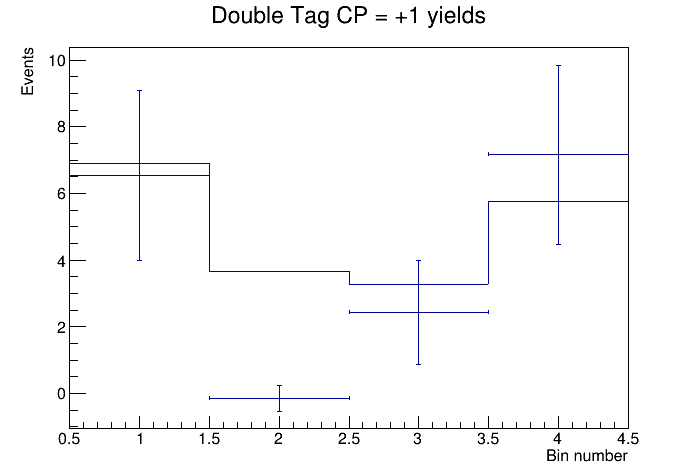
\includegraphics[width=0.8\textwidth]{DoubleTagYieldCPEven.png}
    \caption{$KK$ double tag yield in $KK\pi\pi$ bins}
  \end{figure}
\end{frame}

\begin{frame}{$K_S\pi^0$ double tag yield}
  \begin{figure}
    \centering
    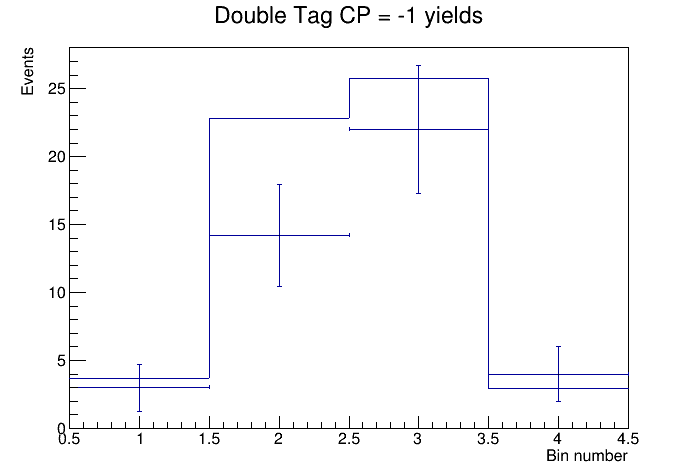
\includegraphics[width=0.8\textwidth]{DoubleTagYieldCPOdd.png}
    \caption{$K_S\pi^0$ double tag yield in $KK\pi\pi$ bins}
  \end{figure}
\end{frame}

\begin{frame}{$K\pi$ double tag yield}
  \begin{figure}
    \centering
    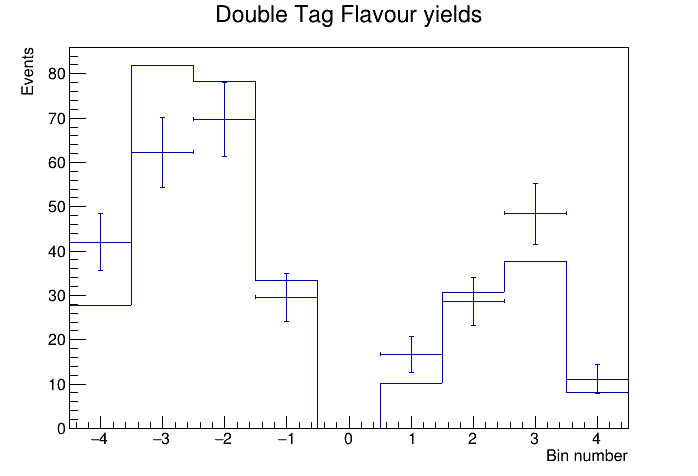
\includegraphics[width=0.8\textwidth]{DoubleTagYieldFlavour.png}
    \caption{$K\pi$ double tag yield in $KK\pi\pi$ bins}
  \end{figure}
\end{frame}

\section{Next steps}
\begin{frame}{Next steps}
  \begin{itemize}
    \setlength\itemsep{2em}
    \item{Yields of other ST modes}
    \item{Yields of other DT modes}
  \end{itemize}
\end{frame}

\end{document}
